%iffalse
\let\negmedspace\undefined
\let\negthickspace\undefined
\documentclass[journal,12pt,onecolumn]{exam}
\usepackage[version=4]{mhchem}
\usepackage{chemformula} % for \ch if needed
\usepackage{chemfig}
\usepackage{chemmacros}
\chemsetup{modules = reactions} % Enables reaction arrows
\usepackage{graphicx}
\graphicspath{ {./images/} }
\usepackage{geometry}
\usepackage{lastpage}
\usepackage{cite}
\usepackage{amsmath,amssymb,amsfonts,amsthm}
\usepackage{enumitem,multicol}
\usepackage{algorithmic}
\usepackage{graphicx}
\usepackage{textcomp}
\usepackage{xcolor}
\usepackage{txfonts}
\usepackage{listings}
\usepackage{enumitem}
\usepackage{mathtools}
\usepackage{gensymb}
\usepackage{comment}
\usepackage[breaklinks=true]{hyperref}
\usepackage{tkz-euclide} 
\usepackage{listings}
\usepackage{gvv}                                        
%\def\inputGnumericTable{}                                 
\usepackage[latin1]{inputenc}                                
\usepackage{color}                                            
\usepackage{array}                                            
\usepackage{longtable}                                       
\usepackage{calc}                                             
\usepackage{multirow}                                         
\usepackage{hhline}                                           
\usepackage{ifthen}                                           
\usepackage{lscape}
\usepackage{tabularx}
\usepackage{array}
\usepackage{float}


\newtheorem{theorem}{Theorem}[section]
\newtheorem{problem}{Problem}
\newtheorem{proposition}{Proposition}[section]
\newtheorem{lemma}{Lemma}[section]
\newtheorem{corollary}[theorem]{Corollary}
\newtheorem{example}{Example}[section]
\newtheorem{definition}[problem]{Definition}
\newcommand{\BEQA}{\begin{eqnarray}}
\newcommand{\EEQA}{\end{eqnarray}}
\newcommand{\define}{\stackrel{\triangle}{=}}
\theoremstyle{remark}

\geometry{margin=1 in}



\setlength{\headheight}{14pt}
\setlength{\headsep}{5pt}
\setlength{\footskip}{20pt}

\begin{document}
\subsection*{Q.1 -- Q.5 carry two marks each.}
\begin{enumerate}
    \item The village was nestled in a green spot,  the ocean and the hills.

    \hfill{(GATE 2023 PE)}\\
\begin{enumerate}
    \item through
    \item in
    \item at
    \item between
\end{enumerate}
\item Disagree : Protest :: Agree :  \\
(word by meaning)

\hfill{(GATE 2023 PE)}\\
\begin{enumerate}
    \item Refuse
    \item Pretext
    \item Recommend
    \item Refute
\end{enumerate}
\item A 'frabjous' number is defined as a 3 digit number with all digits odd, and no two
adjacent digits being the same. For example, 137 is a frabjous number, while 133 is
not. How many such frabjous numbers exist?

\hfill{(GATE 2023 PE)}\\
\begin{enumerate}
    \item 125
    \item 720
    \item 60
    \item 80
\end{enumerate}
\item Which one among the following statements must be TRUE about the mean and the
median of the scores of all candidates appearing for GATE 2023?

\hfill{(GATE 2023 PE)}\\
\begin{enumerate}
    \item The median is at least as large as the mean.
    \item The mean is at least as large as the median.
    \item At most half the candidates have a score that is larger than the median.
    \item At most half the candidates have a score that is larger than the mean.
\end{enumerate}

\item In the given diagram, ovals are marked at different heights (h) of a hill. Which one
of the following options P, Q, R, and S depicts the top view of the hill?
\begin{figure}[H]
    \centering
    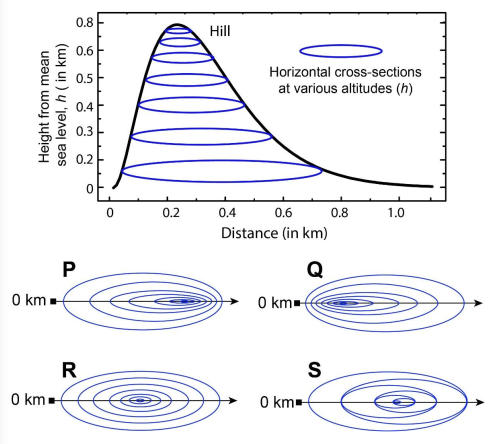
\includegraphics[width=0.5\linewidth]{figs/fig1.png}
    \caption{Figure-1}
    \label{fig:figs/fig1.png}
\end{figure}

\hfill{(GATE 2023 PE)}\\
\begin{enumerate}
    \item P
    \item Q
    \item R
    \item S
\end{enumerate}
\subsection*{Q.6-Q.10 Carry TWO marks Each}

\item Residency is a famous housing complex with many well-established individuals
among its residents. A recent survey conducted among the residents of the complex
revealed that all of those residents who are well established in their respective fields
happen to be academicians. The survey also revealed that most of these
academicians are authors of some best-selling books.
Based only on the information provided above, which one of the following
statements can be logically inferred with certainty?

\hfill{(GATE 2023 PE)}\\
\begin{enumerate}
    \item Some residents of the complex who are well established in their fields are also
authors of some best-selling books.
    \item All academicians residing in the complex are well established in their fields.
    \item Some authors of best-selling books are residents of the complex who are well
established in their fields.
    \item Some academicians residing in the complex are well established in their fields.
\end{enumerate}
\item Ankita has to climb 5 stairs starting at the ground, while respecting the following
rules:
1. At any stage, Ankita can move either one or two stairs up.
2. At any stage, Ankita cannot move to a lower step.
Let F(N) denote the number of possible ways in which Ankita can reach the Nth
stair. For example, F(1) = 1, F(2) = 2, F(3) = 3.
The value of F(5) is

\hfill{(GATE 2023 PE)}\\
\begin{enumerate}
\item 8
\item 7
\item 6
\item 5
\end{enumerate}
  \item   The information contained in DNA is used to synthesize proteins that are necessary
for the functioning of life. DNA is composed of four nucleotides: Adenine (A),Thymine (T), Cytosine (C), and Guanine (G). The information contained in DNA can then be thought of as a sequence of these four nucleotides: A, T, C, and G. DNA has coding and non-coding regions. Coding regions-where the sequence of these nucleotides are read in groups of three to produce individual amino acids-constitute only about 2\% of human DNA. For example, the triplet of nucleotides CCG codes for the amino acid glycine, while the triplet GGA codes for
the amino acid proline. Multiple amino acids are then assembled to form a protein.\\
Based only on the information provided above, which of the following statements
can be logically inferred with certainty?\\
(i)The majority of human DNA has no role in the synthesis of proteins.
(ii)The function of about 98\% of human DNA is not understood.

\hfill{(GATE 2023 PE)}\\
\begin{enumerate}
    \item only (i) 
    \item only (ii)
    \item both (i) and (ii)
    \item neither (i) nor (ii)
\end{enumerate}
\item Which one of the given figures P, Q, R and S represents the graph of the following
function?
 \[
 f(x) = |\,|x+2| - |x-1|\,|
 \]
\begin{figure}[H]
    \centering
    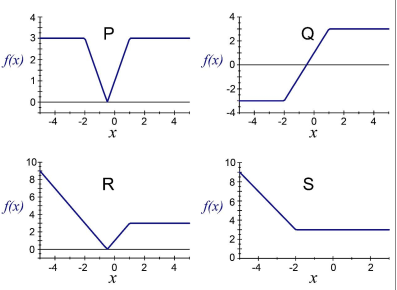
\includegraphics[width=0.5\linewidth]{figs/fig2.png}
    \caption{Figure-2}
    \label{fig:figs/fig2.png}
\end{figure}

\hfill{(GATE 2023 PE)}\\
\begin{enumerate}
    \item P
    \item Q
    \item R
    \item S
\end{enumerate}
\item An opaque cylinder (shown below) is suspended in the path of a parallel beam of
light, such that its shadow is cast on a screen oriented perpendicular to the direction
of the light beam. The cylinder can be reoriented in any direction within the light
beam. Under these conditions, which one of the shadows P, Q, R, and S is NOT
possible?
\begin{figure}[H]
    \centering
    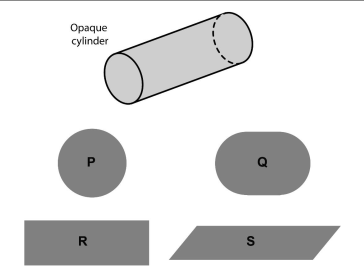
\includegraphics[width=0.5\linewidth]{figs/fig3.png}
    \caption{Figure-3}
    \label{fig:figs/fig3.png}
\end{figure}

\hfill{(GATE 2023 PE)}\\
\begin{enumerate}
    \item P
    \item Q
    \item R
    \item S
\end{enumerate}
\item Let Z1 and Z2 be two arbitrary complex numbers with non-zero modulus. Which of
the following conditions is FALSE?

\hfill{(GATE 2023 PE)}\\
\begin{enumerate}
    \item $\; |z_1 + z_2| \geq |z_1| + |z_2|$
    \item $\; 0 \leq |z_1 + z_2| < \infty$
    \item $\; |z_1 + z_2| \leq |z_1| + |z_2|$
    \item $\; |z_1 z_2| = |z_1||z_2|$
\end{enumerate}
\item In the 4th order Runge-Kutta method for solving ordinary differential equations with
step size h $<$ 1, the ratio of the order of local error to the order of global error is

\hfill{(GATE 2023 PE)}\\
\begin{enumerate}
    \item h
    \item $h^2$
    \item 1/h
    \item 1/$h^2$
\end{enumerate}
\item Which of the following instruments can measure contact angle of a liquid drop
placed on a surface?

\hfill{(GATE 2023 PE)}\\
\begin{enumerate}
    \item Goniometer
    \item Pycnometer
    \item Soxhlet apparatus
    \item Rheometer
\end{enumerate}
\item Which of the following is the primary role of proppants in hydraulic fracturing?

\hfill{(GATE 2023 PE)}\\
\begin{enumerate}
    \item Keep the fractures open during production
    \item Decrease the viscosity of fracturing fluid
    \item Decrease the density of fracturing fluid
    \item Reduce the viscosity of crude oil in reservoir
\end{enumerate}
\item A mixture of a flammable gas and air can ignite ONLY if

\hfill{(GATE 2023 PE)}\\
\begin{enumerate}
    \item the gas concentration is below the limiting oxygen concentration
    \item the gas concentration is above the upper flammable limit
    \item the gas concentration is between the lower and upper flammable limits
    \item the gas concentration is below the lower flammable limit
\end{enumerate}
\item Which of the following relations defines the coefficient of isothermal
compressibility (Cg ) for a gas?
Here, p, T, and v represent the pressure, temperature and volume of the gas,
respectively.

\hfill{(GATE 2023 PE)}\\
\begin{enumerate}
 \item[(A)] $C_T = -\dfrac{1}{V}\left(\dfrac{\partial V}{\partial P}\right)_T$
    \item[(B)] $C_T = -\dfrac{1}{V}\left(\dfrac{\partial P}{\partial V}\right)_T$
    \item[(C)] $C_T = -\dfrac{1}{P}\left(\dfrac{\partial V}{\partial P}\right)_T$
    \item[(D)] $C_T = -\dfrac{1}{P}\left(\dfrac{\partial P}{\partial V}\right)_T$
\end{enumerate}
\item Consider an ideal liquid-vapor mixture at equilibrium having liquid phase mole fraction ${x_i}$ and gas phase mole fraction ${y_i}$ of the component 'i'. If at a given temperature,${P_{vi}}$ is the vapor pressure of pure component 'i' and P is the total
pressure, then the equilibrium ratio ${K_i}$ is

\hfill{(GATE 2023 PE)}\\
    \begin{enumerate}
    \item $k_i = \frac{x_i}{y_i} = \frac{P_{v_i}}{P}$
    \item $k_i = \frac{x_i}{y_i} = \frac{P}{P_{v_i}}$
    \item $k_i = \frac{y_i}{x_i} = \frac{P_{v_i}}{P}$
    \item $k_i = \frac{y_i}{x_i} = \frac{P}{P_{v_i}}$
\end{enumerate}
\item In-situ combustion method for enhanced oil recovery is commonly used for

\hfill{(GATE 2023 PE)}\\
\begin{enumerate}
    \item gas condensate reservoirs
    \item light oil reservoirs
    \item brown oil reservoirs
    \item heavy oil reservoirs
\end{enumerate}
\item Which of the following is a sedimentary rock?

\hfill{(GATE 2023 PE)}\\
\begin{enumerate}
    \item Amphibolite
    \item Chalk
    \item Gabbro
    \item Schist
\end{enumerate}
\item Kerogen is an intermediate compound in the process of petroleum formation in a
sedimentary basin. This is typically classified into four categories (Type-I, Type-II,
Type-III and Type-IV) based on the relative amount of carbon (C), hydrogen (H),
oxygen (O) present in it (shown in the figure below).
Which of the following is the X- axis and Y-axis, respectively?
\begin{figure}[H]
    \centering
    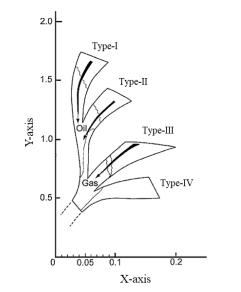
\includegraphics[width=0.5\linewidth]{figs/fig4.png}
    \caption{Figure-4}
    \label{fig:figs/fig4.png}
\end{figure}

\hfill{(GATE 2023 PE)}\\
\begin{enumerate}
    \item H:C ratio and O:C ratio
    \item O:C ratio and H:C ratio
    \item C:H ratio and C:O ratio
    \item C:O ratio and C:H ratio
\end{enumerate}
\item The response of a four-arm caliper (dual caliper) log in a drilled section is shown in
the figure below. The borehole features associated with the three identified sections
P, Q, and R are
\begin{figure}[H]
    \centering
    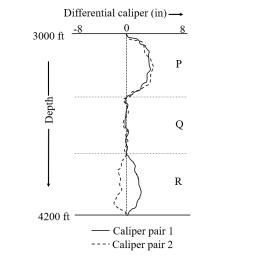
\includegraphics[width=0.5\linewidth]{figs/fig5.png}
    \caption{Figure-5}
    \label{fig:figs/fig5.png}
\end{figure}

\hfill{(GATE 2023 PE)}\\
\begin{enumerate}
    \item P: washout; Q: in-gauge hole; R: key-seat
    \item P: key-seat; Q: in-gauge hole; R: washout
    \item P: under-gauge hole; Q: in-gauge hole; R: washout
    \item P: dog-leg; Q: in-gauge hole; R: key-seat
\end{enumerate}
\item Which of the following is necessary for the generation of electrokinetic potential
across well-bore and permeable rock formation?

\hfill{(GATE 2023 PE)}\\
\begin{enumerate}
    \item Salinity gradient
    \item Pressure gradient
    \item Shale membrane
    \item Mud cake
\end{enumerate}
\item A first arrival amplitude of the Cement Bond Log (CBL) of a cased hole section is
given in the figure. The identified depth intervals P, Q, and R represent
\begin{figure}[H]
    \centering
    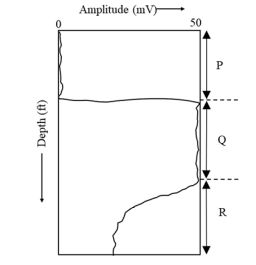
\includegraphics[width=0.5\linewidth]{figs/fig6.png}
    \caption{Figure-6}
    \label{fig:figs/fig6.png}
\end{figure}

    \hfill{(GATE 2023 PE)}\\
\begin{enumerate}
    \item P: not cemented; Q: partially cemented; R: well-cemented
    \item P: not cemented; Q: well-cemented; R: partially cemented
    \item P: partially cemented; Q: not cemented; R: well-cemented
    \item P: well-cemented; Q: not cemented; R: partially cemented
\end{enumerate}
\item Contact angle measurements are often performed on smooth surfaces to gain
information about the wettability of a surface. The interfacial tensions between
Which of the following expressions describes the contact angle, $\theta$?

\begin{figure}[H]
    \centering
    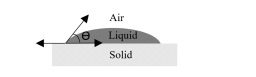
\includegraphics[width=0.5\linewidth]{figs/fig7.png}
    \caption{Figure-7}
    \label{fig:figs/fig7.png}
\end{figure}

 \hfill{(GATE 2023 PE)}\\
\begin{enumerate}
     \item $\cos \Theta = \frac{\gamma_{AS} - \gamma_{SL}}{\gamma_{LA}}$
    \item $\cos \Theta = \frac{\gamma_{SL} - \gamma_{AS}}{\gamma_{LA}}$
    \item $\cos \Theta = \frac{\gamma_{LA} - \gamma_{AS}}{\gamma_{SL}}$
    \item $\cos \Theta = \frac{\gamma_{LA} - \gamma_{SL}}{\gamma_{AS}}$
\end{enumerate}
\item Which of the following offshore rigs has the HIGHEST water depth of operation?

 \hfill{(GATE 2023 PE)}\\
\begin{enumerate}
    \item Submersible drilling barge
    \item Jackup rigSemi-submersible rig
    \item Jacket platform
    \item Semi-submersible rig
\end{enumerate}
\item Consider an immiscible liquid mixture of n-decane and water containing fully
dissociated NaCl. The number of degrees of freedom for this system is

\hfill{(GATE 2023 PE)}\\
\begin{enumerate}
    \item 3
    \item 4
    \item 5
    \item 2
\end{enumerate}
\item The mean free path of the gas molecule is $10^{-6} mm$, while the pore size of the rock
is $10^{-3} mm$. Which of the following statements is TRUE?

\hfill{(GATE 2023 PE)}\\
\begin{enumerate}
    \item The Knudsen number is 103 and the continuum principle would be applicable
    \item The Knudsen number is 10-3 and the continuum principle would be applicable
    \item The Knudsen number is 103 and the continuum principle would not be applicable
    \item The Knudsen number is 10-3 and the continuum principle would not be applicable
\end{enumerate}
\item Which of the following is/are the route(s) by which a toxic substance may enter a human body?

\hfill{(GATE 2023 PE)}\\
\begin{enumerate}
    \item Ingestion
    \item Inhalation
    \item Perspiration
    \item Asphyxiation
\end{enumerate}
\item Select ALL the safety system(s) that is/are required in an offshore platform.

\hfill{(GATE 2023 PE)}\\
\begin{enumerate}
    \item Permit to work system
    \item Fire and gas alarms
    \item Lock out-tag out
    \item Financial monitoring system
\end{enumerate}
\item Polymer flooding enhances oil recovery from an oil reservoir by

\hfill{(GATE 2023 PE)}\\
\begin{enumerate}
    \item increasing the mobility ratio
    \item reducing the mobility ratio
    \item reducing the viscous fingering
    \item increasing the viscous fingering
\end{enumerate}
\item Which is/are the thermodynamic inhibitor(s) for natural gas hydrate?

\hfill{(GATE 2023 PE)}\\
\begin{enumerate}
    \item Tetrahydrofuran
    \item Sodium chloride
    \item Ethylene glycol
    \item Tetra n-butyl ammonium bromide
\end{enumerate}
\item Which of the following hydrocarbon trap(s) is/are a result of sedimentary facies
changes?

\hfill{(GATE 2023 PE)}\\
\begin{enumerate}
    \item Salt dome
    \item Unconformity
    \item Pinch out
    \item Sand lens
\end{enumerate}
\item Which of the following option(s) is/are indication(s) of a well kick?

\hfill{(GATE 2023 PE)}\\
\begin{enumerate}
    \item Decrease in mud pit volume
    \item Increase in mud pit volume
    \item Decrease in pump pressure
    \item Increase in pump pressure
\end{enumerate}
\item 
Let $\mathbf{X} = 
\begin{bmatrix}
x_{11} & x_{12} & x_{13} \\
x_{21} & x_{22} & x_{23} \\
x_{31} & x_{32} & x_{33}
\end{bmatrix}
$ be a $3 \times 3$ matrix.

The determinant of matrix $\mathbf{X}$ is 5.

The determinant of matrix $\mathbf{Y} = 
\begin{bmatrix}
x_{11} & x_{12} & x_{13} \\
2x_{21} & 2x_{22} & 2x_{23} \\
3x_{31} & 3x_{32} & 3x_{33}
\end{bmatrix}
$ is \underline{\hspace{2cm}}.

\hfill{(GATE 2023 PE)}\\
\item 
Consider a vector field $\vec{V} = x\hat{i} + 2y^2\hat{j} + 0.5z\hat{k}$, where $\hat{i},\ \hat{j},\ \hat{k}$ are the unit vectors in $x$, $y$ and $z$ directions, respectively.

The divergence of $\vec{V}$ at the point $(1, 2, 1)$ is \underline{\hspace{2cm}} (rounded to one decimal place).

\hfill{(GATE 2023 PE)}\\
\subsection*{Q.36-Q.65 Carry TWO marks Each}
\item  The value of 
\[
\int_{0}^{\pi} \int_{-1}^{1} r^{2} \sin^{2}\theta \, dr \, d\theta
\]
is

\hfill{(GATE 2023 PE)}\\
\begin{enumerate}
\item[(A)] $\dfrac{\pi}{4}$
\item[(B)] $\dfrac{\pi}{8}$
\item[(C)] $\dfrac{\pi}{16}$
\item[(D)] $\dfrac{\pi}{3}$
\end{enumerate}
\item Consider the following accident scenario:
Failure of a drain connection on a rich oil line at the base of an absorber tower in
a gas producing plant allowed the release of rich oil and gas. The resulting vapor
cloud ignited from the ignition system of an engine-driven recompressor. The
absorber tower eventually collapsed across a pipe rack. The breakage of the
pipelines added more fuel to the fire and lead to the total destruction of the plant.
The resulting fire burnt for 3 days.
Match the three steps of any accident (initiation, propagation, and termination) to
the events that occurred in the above scenario.
\begin{center}
\begin{tabular}{ll}
    \textbf{Group I} & \textbf{Group II} \\
    P. Ferrite & 1. Hexagonal Close Packed (HCP) \\
    Q. Austenite & 2. Body Centered Cubic (BCC) \\
    R. Martensite & 3. Body Centered Tetragonal (BCT) \\
    & 4. Face Centered Cubic (FCC)
\end{tabular}
\end{center}

\hfill{(GATE 2023 PE)}\\
\begin{enumerate}
    \item P-I; Q-III; R-II
    \item P-II; Q-I; R-III
    \item P-II; Q-III; R-I
    \item P-I; Q-II; R-III
\end{enumerate}
\item A centrifugal pump running at 500 rpm delivers 60 liters/minute with a head of
50 m. At the same efficiency, if the rotational speed is increased to 1000 rpm, the
discharge rate and head would respectively be

\hfill{(GATE 2023 PE)}\\
\begin{enumerate}
    \item 120 liters/minute and 200 m
    \item 120 liters/minute and 100 m
    \item 60 liters/minute and 200 m
    \item60 liters/minute and 100 m
\end{enumerate}
\item Match the flow regimes associated with a vertically fractured well in a reservoir.
\begin{figure}[H]
    \centering
    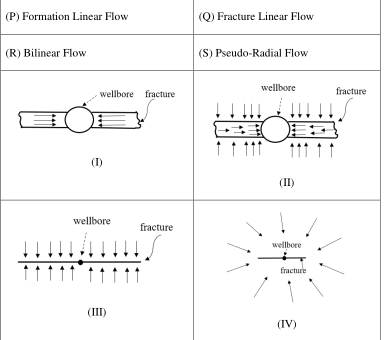
\includegraphics[width=0.5\linewidth]{figs/fig8.png}
    \caption{Figure-8}
    \label{fig:figs/fig8.png}
\end{figure}

\hfill{(GATE 2023 PE)}\\
\begin{enumerate}
    \item P-I; Q-III; R-II; S-IV
    \item P-III; Q-I; R-II; S-IV
    \item P-III; Q-I; R-IV; S-II
    \item P-I; Q-II; R-III; S-IV
\end{enumerate}
\item The figure shows a schematic representation of the organic solid phase diagram
for wax, hydrate and asphaltene deposition around the bubble point of a sample
reservoir fluid. Arrowheads indicate the stable region for a corresponding organic
solid.
\begin{figure}[H]
    \centering
    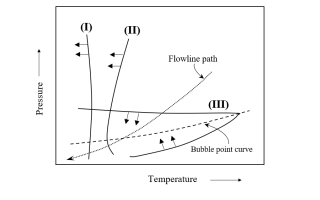
\includegraphics[width=0.5\linewidth]{figs/fig9.png}
    \caption{Figure-9}
    \label{fig:figs/fig9.png}
\end{figure}
Match the phase diagram with organic solids.

\hfill{(GATE 2023 PE)}\\
\begin{enumerate}
    \item I - Wax; II - Hydrate; III - Asphaltene
    \item I - Hydrate; II - Asphaltene; III - Wax
    \item I - Asphaltene; II - Hydrate; III - Wax
    \item I - Hydrate; II - Wax; III - Asphaltene
\end{enumerate}
\item Schematic of phase diagrams for a pure gas hydrate system of methane (CH4),
carbon dioxide (CO2), hydrogen sulphide (H2S) and nitrogen (N2) between the
lower and upper quadruple points are shown in figure. Arrowheads indicate the
stable hydrate region for a particular gas hydrate system.
\begin{figure}[H]
    \centering
    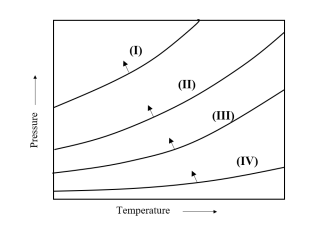
\includegraphics[width=0.5\linewidth]{figs/fig10.png}
    \caption{Figure-10}
    \label{fig:figs/fig10.png}
\end{figure}
Match the phase diagram with the corresponding pure gas hydrate.

\hfill{(GATE 2023 PE)}\\
\begin{enumerate}
   \item I -- CH$_4$; II -- N$_2$; III -- CO$_2$; IV -- H$_2$S
\item I -- H$_2$S; II -- CH$_4$; III -- CO$_2$; IV -- N$_2$
\item I -- N$_2$; II -- CH$_4$; III -- H$_2$S; IV -- CO$_2$
\item I -- N$_2$; II -- CH$_4$; III -- CO$_2$; IV -- H$_2$S
\end{enumerate}
\item Match the entries between Group-I and Group-II for the seismic data acquisition, processing and interpretation.
\begin{figure}[H]
    \centering
    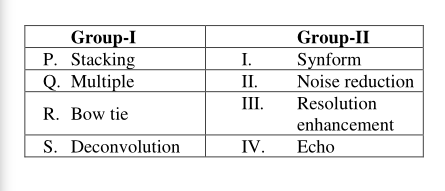
\includegraphics[width=0.5\linewidth]{figs/fig11.png}
    \caption{Figure-11}
    \label{fig:figs/fig11.png}
\end{figure}

\hfill{(GATE 2023 PE)}\\
\begin{enumerate}
    \item P-II; Q-IV; R-I; S-III
    \item P-II; Q-I; R-IV; S-III
    \item P-III; Q-IV; R-I; S-II
    \item P-III; Q-I; R-IV; S-II
\end{enumerate}
\item A build-up test is characterized by production at constant rate over time, $t_p$, 
followed by shut-in period of $\Delta t$. A plot of shut-in bottom hole pressure ($P_{ws}$) with 
\[
\log \left( \frac{t_p + \Delta t}{\Delta t} \right)
\]
for pressure build-up test data is shown in the figure.
\begin{figure}[H]
    \centering
    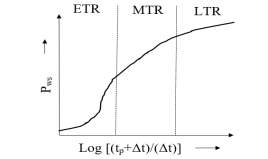
\includegraphics[width=0.5\linewidth]{figs/fig12.png}
    \caption{Figure-12}
    \label{fig:figs/fig12.png}
\end{figure}

Which of the following statement(s) is/are TRUE?

\hfill{(GATE 2023 PE)}\\
\begin{enumerate}
\item[(A)] Early Time Region (ETR): Pressure build-up data is affected by reservoir 
boundaries and other reservoir heterogeneities such as sealing faults
\item[(B)] Middle Time Region (MTR): Pressure build-up data is reached after end of the 
wellbore storage and the pressure transient has entered the virgin reservoir
\item[(C)] Late Time Region (LTR): Pressure build-up data is affected by reservoir 
boundaries and other reservoir heterogeneities such as sealing faults
\item[(D)] Middle Time Region (MTR): Pressure build-up data is affected by reservoir 
boundaries and other reservoir heterogeneities such as sealing faults
\end{enumerate}
\item Select the statement(s) that is/are TRUE.

\hfill{(GATE 2023 PE)}\\
\begin{enumerate}
    \item Combustion always occurs in the vapor phase
    \item Combustion cannot occur if air is absent
    \item Flash point is the lowest temperature at which a vapor above a liquid will
continue to burn once ignited
    \item The distinction between a fire and explosion is in their rate of energy release
\end{enumerate}
\item Using Simpson\'s one-third rule (with step size h = 0.25), the area under the curve
y = $1/e^x$, from x = 0 to x = 1 is (rounded to two decimal places).

\hfill{(GATE 2023 PE)}\\
\item The directional derivative of f=$x^3+4y^2+z^2$ at the point P (2, 1, 3) in thedirection of the vector V=3i-4k is (rounded to one decimal place).

\hfill{(GATE 2023 PE)}
\item A switch-over event in a producing well occasionally results in a reportable oil
leak. An analysis of the data shows that the chance of a reportable leak is 1 in 500
switch-over events. It is observed that 10 switch-over events occur every day.
If the occurrence of a reportable leak follows a Poisson distribution, the number
of days in a year (of 365 days) with no reportable oil leaks from switch-over events is

\hfill{(GATE 2023 PE)}
\item Figure shows an inextensible catenary mooring cable in still water. The
submerged weight (per meter length), and the anchor radius (x) are 100 kg/m and
50 m, respectively. If horizontal tension (Th ) in the catenary is 1600 kg, the
catenary length (AB) is  (rounded to two decimal places).

\hfill{(GATE 2023 PE)}
\item An empty steel pipeline with massless endcaps has an outer diameter, D, and
thickness, t. The density of steel is 7850 kg/m3 . The critical D/t ratio at which the
pipeline starts floating in seawater of density 1025 kg/m3 is

\hfill{(GATE 2023 PE)}
\item Consider the flow of oil and water in one-dimensional porous medium, with 
$k_{ro}^0 = 1$, $k_{rw}^0 = 0.2$, $S_{wr} = 0.2$ and $S_{or} = 0.4$, where $k_{ro}^0$ and $k_{rw}^0$ are the end point
relative permeabilities of oil and water, respectively; $S_{or}$ and $S_{wr}$ are the residual
saturations of oil and water, respectively. The viscosities of oil and water are $5$ cP
and $1$ cP, respectively. $k_{ro}$ and $k_{rw}$ are the relative permeabilities of oil and water,
respectively, at a given water saturation $(S_w)$. Following relations are valid.
\[
k_{ro} = k_{ro}^0 \bigl(1 - S_w^*\bigr), \qquad
k_{rw} = k_{rw}^0 \, S_w^*, \qquad
S_w^*=\frac{S_w-S_{wr}}{1-S_{or}-S_{wr}}.
\]

The total relative mobility (oil relative mobility + water relative mobility) at the water
saturation of $0.4$ is \underline{\hspace{2cm}}~cP$^{-1}$ (rounded to one decimal place)

\hfill{(GATE 2023 PE)}
\item A binary mixture of n-butane (C4H10) and n-pentane (C5H12) is under
thermodynamic equilibrium at 180 oF and 95 psia. The vapor pressures of pure
$C_4H_{10}$ and pure C5H12 at 180 oF are 160 psia and 54 psia, respectively.
Assuming ideal solution behavior 
the mole fraction of the n-butane in the gas phase is

\hfill{(GATE 2023 PE)}
\item A highly permeable reservoir with initial reservoir pressure of 3000 psi is under
active water drive from a surrounding large aquifer. The final stabilized reservoir
pressure is 2500 psi. Following data associated with the reservoir at 2500 psi are
given.\\
Oil production rate = 30,000 STB/day\\
Water production rate = 0 STB/day\\
Oil formation volume factor, Bo = 1.5 bbl/STB\\
Gas formation volume factor, Bg = 0.00070 bbl/scf\\
Water formation volume factor, Bw = 1 bbl/STB\\
Producing Gas to Oil Ratio, GOR = 850 scf/STB\\
Gas solubility, Rs = 700 scf/STB\\
(bbl: reservoir barrel, STB: Stock tank barrel, scf: standard cubic feet)\\
If the reservoir pressure and the reservoir production rates remain constant, the
water influx rate is

\hfill{(GATE 2023 PE)}
\item A volumetric undersaturated solution gas drive reservoir (without gas cap, no
water influx, and with no initial gas saturation) has an initial water saturation of
15\% which remains unchanged during production. After the production of 10\%
of the initial oil (measured at surface conditions), the oil formation volume factor
(Bo) is reduced from its initial value of 1.4 bbl/STB to 1.2 bbl/STB.\\
(bbl: reservoir barrel, STB: Stock tank barrel)\\
The final gas saturation in percentage is
\hfill{(GATE 2023 PE)}
\item After well completion, a discovery well in an oil reservoir is produced for a short
period and then closed for pressure build-up test. The production history before
shut-in is given below.
\begin{tabular}{|c|c|c|}
     \hline
     \textbf{Mineral} & \textbf{Modal abundance \brak{\%}} & \textbf{Partition coefficient}\\
     \hline
     Clinopyroxene & $45$ & $0.506$ \\
      \hline
      Orthopyroxene & $40$ & $0.42$ \\
      \hline
      Olivine & $10$ & $0.045$ \\
      \hline
      Plagioclase & $05$ & $0.019$ \\
      \hline
\end{tabular}
The Horner\'s pseudo-producing time $t_{pH}$, is
\hfill{(GATE 2023 PE)}
\item A compressional acoustic wave takes 55$\mu$s to travel 0.3048 m through a rock
formation having bulk modulus of 37.5 GPa and shear modulus of 31 GPa. The
bulk density of the rock is

\hfill{(GATE 2023 PE)}
\item A gamma ray log run across a sand-shale sequence recorded maximum and
minimum values of 70 API unit and 30 API unit, respectively. A bed in this
sequence has a gamma log value of 50 API unit.
Assuming a linear relationship between shale index and shale volume, the volume
fraction of shale in the bed is \underline{\hspace{2cm}} (rounded to one decimal place).

\hfill{(GATE 2023 PE)}
\item The resistivity reading of a flushed zone across a permeable formation (drilled
with water-based mud) is 20 ohm.m. Laboratory analysis shows that the resistivity
of the core plug (100\% saturated with a NaCl brine) from the same formation is
6 ohm.m. The resistivity of the NaCl brine is 0.6 ohm.m.\\
If the resistivity of the mud filtrate is 0.9 ohm.m and Archie/'s saturation exponent is
2, then the estimated residual hydrocarbon saturation (in percentage) in the
flushed zone is \underline{\hspace{2cm}}  (rounded to two decimal places).

\hfill{(GATE 2023 PE)}
\item Consider a micellar displacement process in a homogeneous reservoir with a
porosity of 30\%. The volume of the microemulsion slug to be injected is 4\% of
the pore volume. The slug contains 4 vol\% surfactant. The density of the rock and
the surfactant is 2.7 g/$cm^3$ and 1.1 g/$cm^3$, respectively.\\
Assuming that the average surfactant adsorption is 0.25 mg/g of the reservoir rock,
the fraction of the injected surfactant that will be adsorbed is \underline{\hspace{2cm}} 
(rounded to two decimal places).

\hfill{(GATE 2023 PE)}
\item A kill mud of appropriate density is required to be injected in a well such that the
shut-in pressure is 6.8 x 106 Pa at a depth of 3500 m. Here, the shut-in pressure is
the quantity by which the bottom-hole pressure exceeds the hydrostatic pressure
of the original mud at the given depth. The density of the original mud is
1100 kg/$m^3$.\\
The density of the kill mud is  \underline{\hspace{2cm}}  kg/$m^3$ (rounded to two decimal places).

\hfill{(GATE 2023 PE)}
\item A non-Newtonian drilling fluid is placed between two flat parallel rectangular
plates having an area of 10 cm2 each. The bottom plate is fixed and the vertical
distance between the two plates is 1 cm, as shown in the figure. A force of 300
dyne is required to initiate the motion of the upper plate. A force of 600 dyne is
needed to keep the upper plate in motion at a constant velocity of 10 cm/s. Assume
that the following relationship holds for the drilling fluid.
\[
\tau_{yx} = \mu_p \dot{\gamma} + \tau_{yx}^0
\]

where, $\tau_{yx}$ is the shear stress, $\tau_{yx}^0$ is the minimum shear stress to initiate fluid flow; 
$\mu_p$ is the Bingham plastic viscosity; and $\dot{\gamma}$ is the shear rate.

\begin{figure}[H]
    \centering
    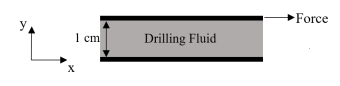
\includegraphics[width=0.5\linewidth]{figs/fig13.png}
    \caption{Figure-13}
    \label{fig:figs/fig13.png}
\end{figure}

The Bingham plastic viscosity of fluid is \underline{\hspace{2cm}}  dyne.s/$cm^2$ (rounded to
nearest integer).

\hfill{(GATE 2023 PE)}
\item Crude oil having density and viscosity of 850 kg/m3 and 2 x 10-3 Pa.s, respectively,
is flowing at an average velocity of 0.35 m/s through a horizontal capillary tube.
The inside diameter and length of the capillary tube are 2.5 x 10-3 m and 0.30 m,
respectively. The Fanning friction factor, f, is given by,

       f = 16/Re

where, Re is the Reynolds number.
The pressure drop across the capillary tube is  \underline{\hspace{2cm}} Pa (rounded to one decimal place).

\hfill{(GATE 2023 PE)}
\item An oil droplet is to be mobilized by injecting water through a pore throat. The oil-
water interface has the rear radius of curvature (rA) of 25 x 10-6 m and a forward
radius of curvature (rB) of 5 x 10-6 m as shown in the figure. Assume that the pore
is completely water wet (wetting contact angle is zero) and the interfacial tension
between oil and water is 0.025 N/m.
\begin{figure}[H]
    \centering
    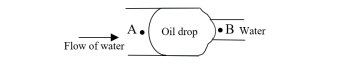
\includegraphics[width=0.75\linewidth]{figs/fig14.png}
    \caption{Figure-14}
    \label{fig:figs/fig14.png}
\end{figure}
The magnitude of the minimum pressure drop required to mobilize the trapped oil
droplet is \underline{\hspace{2cm}}N/$m^2$ (rounded to nearest integer).

\hfill{(GATE 2023 PE)}
\item A four-column semi-submersible floater is located offshore. The diameter of each
column is 5 m. Consider the total displaced weight of seawater of the semi-
submersible as 4000 tonnes. Assume added mass contribution as 50\% of the semi-submersible weight, and seawater density as 1025 kg/$m^3$.\\
(Acceleration due to gravity = 9.81 m/$s^2$)\\
The natural period of oscillation of the floater in vertical mode is  \underline{\hspace{2cm}}
seconds (rounded to one decimal place).

\hfill{(GATE 2023 PE)}
\item A shell and tube heat exchanger is used for cooling crude oil from 400 K to 360 K.
Crude oil flows through the tube at 3650 kg/h. Water enters the shell side at 310 K
and has a flow rate of 1600 kg/h. Assume the heat capacity of crude oil and water as 2.5 kJ/kg. K and 4.187 kJ/kg. K, respectively.\\
If the overall heat transfer coefficient is 300 W/$m^2$ . K and the streams are countercurrent, the heat transfer area required is\underline{\hspace{2cm}} $m^2$ (rounded to one decimal place).

\hfill{(GATE 2023 PE)}
\item An underwater riser with an outer diameter of 250 mm and wall thickness of
20 mm is subjected to tension and pressure. The effective tension is 1200 kN
wherein the internal and external pressures of the riser are 25 MPa and 6 MPa, respectively.\\
The true wall tension in the riser is \underline{\hspace{2cm}} x$10^6$ N (rounded to two decimal places).

\hfill{(GATE 2023 PE)}















\end{enumerate}
\end{document}